\begin{frame}\frametitle{Informações Gerais}

\begin{itemize}
\item
  Analisar o comportamento do usuário
  {[}Apontador{]}{[}www.apontador.com{]} em relação a concessionárias
\item
  Compreender as diferenças do comportamento deste tipo de usuário ao
  usuário comum
\item
  Compreender a distribuição temporal e espacial das buscas por
  concessionárias
\item
  Analisar a existência similaridades de marcas pelas buscas dos
  usuários
\end{itemize}

\begin{block}{Composição da base}

\ctable[pos = H, center, botcap]{cc}
{% notes
}
{% rows
\FL
Marca & Quantidade
\ML
GM & 583
\\\noalign{\medskip}
Row2 Cell1 & Row2 Cell2
\LL
}

\end{block}

\begin{block}{Evolução das visitas de usuários por marca}

\end{block}

\begin{block}{Comportamento padrão do usuário}

\begin{figure}[htbp]
\centering
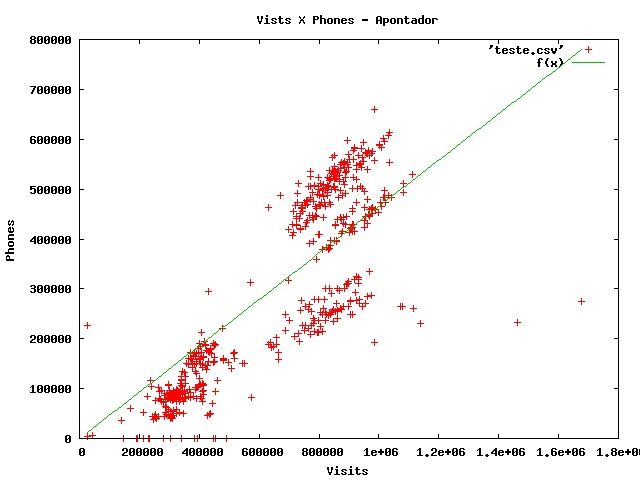
\includegraphics{./total.jpg}
\caption{image}
\end{figure}

\end{block}

\begin{block}{Comportamento na categoria: Concessionária}

\begin{figure}[htbp]
\centering
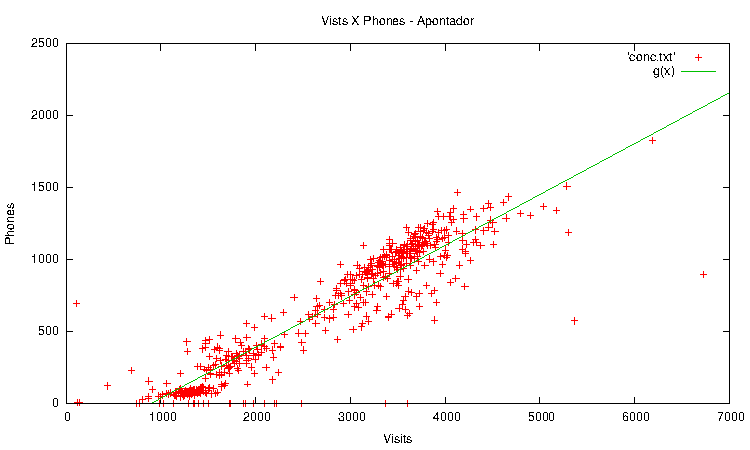
\includegraphics{conc.pdf}
\caption{image}
\end{figure}

\end{block}

\begin{block}{Resultados}

$f(x) = ax + b$

\ctable[pos = H, center, botcap]{lll}
{% notes
}
{% rows
\FL
 & Total & Concessionárias
\ML
a & 0.4649 & 0.3540
\\\noalign{\medskip}
b & 0.7391 & -318.221
\LL
}

A primeira informação que podemos tirar é que o número de ver telefones
para o subgrupo concessárias é proporcionalmente menor que o geral. O
usuário comum é 31\% mais provável a ver telefone que o que procura
concessionárias

\end{block}

\end{frame}

\begin{frame}\frametitle{Comportamento de avaliação do usuário}

\begin{block}{Avaliação positivas - Word Cloud}

\begin{figure}[htbp]
\centering
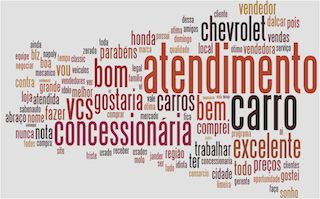
\includegraphics{tagpositivo.png}
\caption{image}
\end{figure}

\end{block}

\begin{block}{Avaliação negativas - Word Cloud}

\begin{figure}[htbp]
\centering
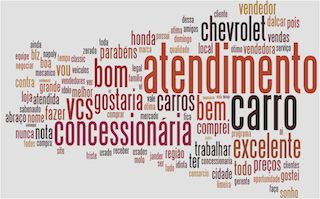
\includegraphics{tagpositivo.png}
\caption{image}
\end{figure}

\end{block}

\end{frame}
